\documentclass[border=10pt]{standalone}
\usepackage{verbatim}
\usepackage{pgfplots}
\usetikzlibrary{spy}
\pgfplotsset{compat=1.14}

% stars_count = 1024 * 32;
% max_time = 1
% max_step = 0.01
% ratio = {0.1, 0.5, 1, 2, 4, 16, 64, 256, 1024};

\begin{document}

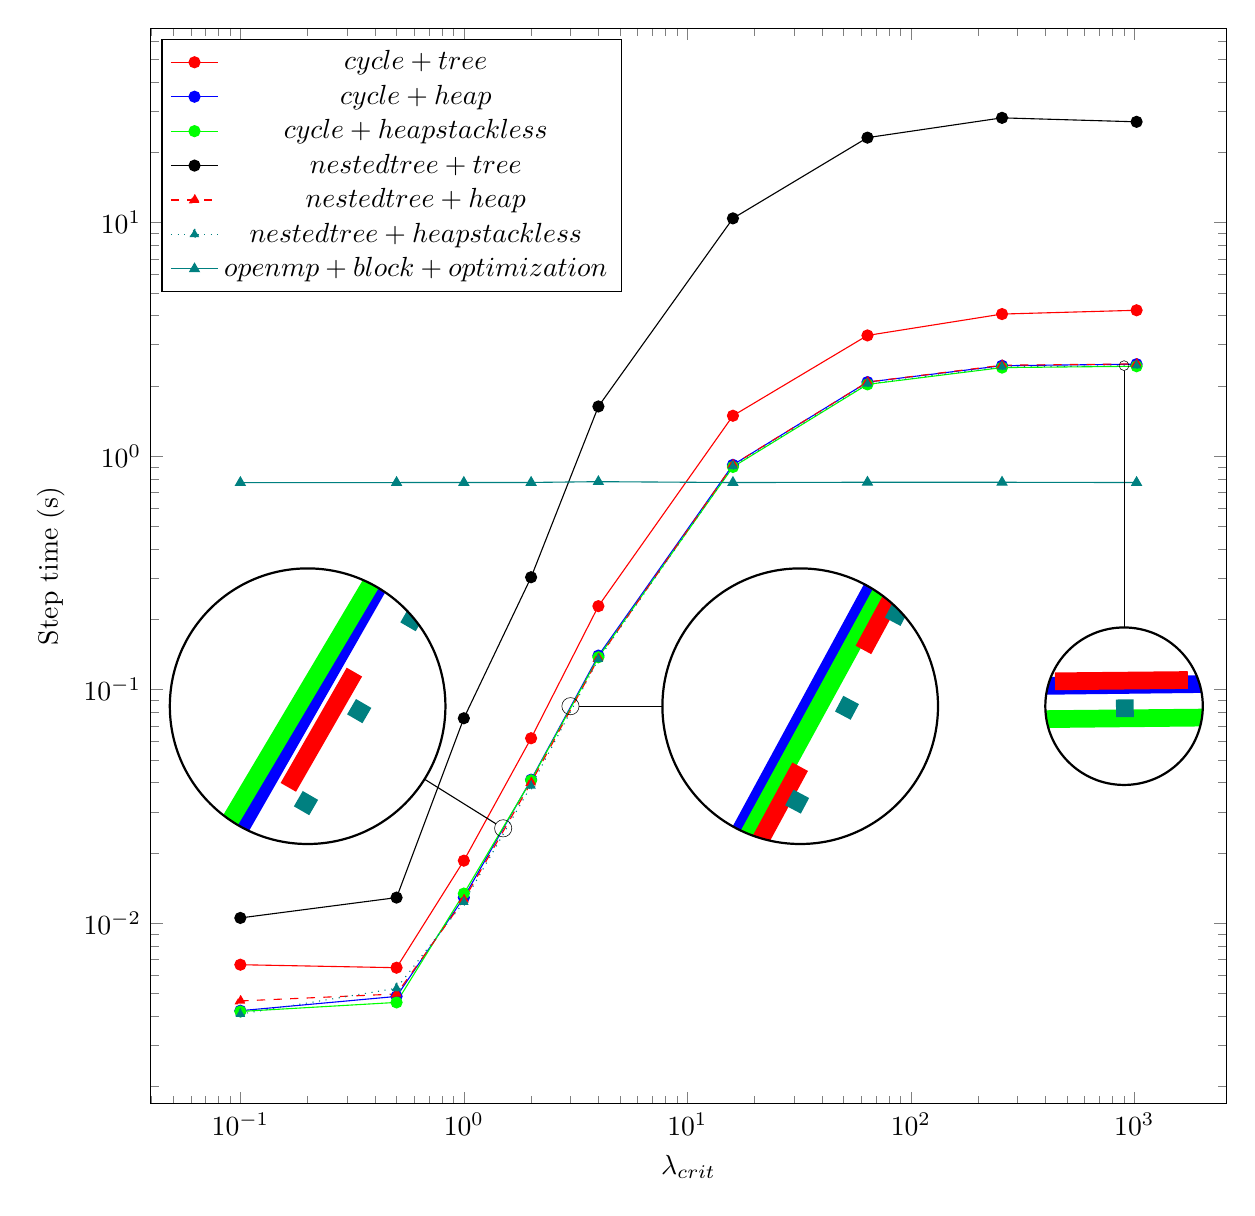
\begin{tikzpicture}[spy using outlines={circle, magnification=16,connect spies}]
\begin{loglogaxis}[
    height=6in,
    width=6in,
    xlabel=$\lambda_{crit}$,
    ylabel=Step time (s),
    legend style={at={(0.01,0.99)},anchor=north west}
]
\addplot [red,mark=*,solid] coordinates { (0.1, 0.006646) (0.5, 0.006453) (1, 0.01854) (2, 0.06199) (4, 0.228) (16, 1.49) (64, 3.289) (256, 4.06) (1024, 4.215) };
\addplot [blue,mark=*,solid] coordinates { (0.1, 0.004223) (0.5, 0.004862) (1, 0.01289) (2, 0.04119) (4, 0.14) (16, 0.918) (64, 2.076) (256, 2.44) (1024, 2.478) };
\addplot [green,mark=*,solid] coordinates { (0.1, 0.004191) (0.5, 0.004583) (1, 0.0134) (2, 0.04093) (4, 0.1377) (16, 0.8993) (64, 2.03) (256, 2.395) (1024, 2.427) };
\addplot [black,mark=*,solid] coordinates { (0.1, 0.01054) (0.5, 0.01288) (1, 0.07549) (2, 0.3032) (4, 1.633) (16, 10.43) (64, 23.12) (256, 28.1) (1024, 27.02) };
\addplot [red,mark=triangle*,dashed] coordinates { (0.1, 0.004649) (0.5, 0.00498) (1, 0.01259) (2, 0.04002) (4, 0.1361) (16, 0.9188) (64, 2.077) (256, 2.452) (1024, 2.484) };
\addplot [teal,mark=triangle*,dotted] coordinates { (0.1, 0.004085) (0.5, 0.005269) (1, 0.01231) (2, 0.03872) (4, 0.1351) (16, 0.9056) (64, 2.041) (256, 2.411) (1024, 2.442) };
\addplot [teal,mark=triangle*,solid] coordinates { (0.1, 0.7709) (0.5, 0.7711) (1, 0.7717) (2, 0.772) (4, 0.7779) (16, 0.7712) (64, 0.7735) (256, 0.7733) (1024, 0.7714) };

\legend{$cycle+tree$,$cycle+heap$,$cycle+heap stackless$,$nested tree+tree$,$nested tree+heap$,$nested tree+heap stackless$,$openmp+block+optimization$};

\coordinate (spypoint0) at (axis cs:1.5, 0.0255);
\coordinate (spyviewer0) at (axis cs:0.2, 0.085);
\spy[width=3.5cm,height=3.5cm] on (spypoint0) in node [fill=white] at (spyviewer0);

\coordinate (spypoint1) at (axis cs:900, 2.442);
\coordinate (spyviewer1) at (axis cs:900,0.085);
\spy[width=2cm,height=2cm] on (spypoint1) in node [fill=white] at (spyviewer1);

\coordinate (spypoint2) at (axis cs:3, 0.085);
\coordinate (spyviewer2) at (axis cs:32, 0.085);
\spy[width=3.5cm,height=3.5cm] on (spypoint2) in node [fill=white] at (spyviewer2);

\end{loglogaxis}
\end{tikzpicture}

\end{document}
